
\chapter{Emodialisi: modello originario}
Il modello di equazioni differenziali  per la simulazione di una seduta di emodialisi è un modello bi-compartimentale (intra- ed extra-cellulare) per quanto riguarda gli scambi di massa e tri-compartimentale (intracellulare, interstiziale, plasmatico) per gli scambi di volume. Il volume plasmatico e quello interstiziale sono considerati complianti e pertanto bisogna considerare anche le relative variazioni di pressione.\\
\newline
Per le variazioni di massa\footnote{La (s) all'apice indica che l'equazione deve essere scritta per ogni soluto considerato} si ha:

\begin{align}
		\frac{dM_{ic}^{(s)}}{dt} &= \Phi_{ic}^{(s)}                \label{dMic}\\
		\frac{dM_{ex}^{(s)}}{dt} &= -\Phi_{ic}^{(s)} -\Phi_d^{(s)} \label{dMex}
\end{align}
\newline
per le variazioni di volume:
\begin{align}
		\frac{dV_{ic}}{dt} &= Q_{ic}\\
		\frac{dV_{is}}{dt} &= Q_{Fa} -Q_{Rv} -Q_{ic}\\
		\frac{dV_{pl}}{dt} &= Q_{Rv}-Q_{Fa} -Q_{F}
\end{align}
\newline
per le variazioni di pressione:
\begin{align}
		\frac{dP_{ac}}{dt} &= \frac{1}{C_c} \frac{dV_{pl}}{dt}\\
		\frac{dP_{is}}{dt} &= E_{is}\frac{dV_{is}}{dt}
\end{align}
\newline
dove:

\begin{align}
		&\Phi_{ic}^{(s)}& &=& &-k(C_{ic} - \beta C_{is})+ Q_{ic}(1-\sigma)\frac{C_{ic}+C_{is}}{2} \label{Phi_ic} \\
		&\Phi_d^{(s)}&    &=& &D\biggl(\alpha \frac{C_{pl}}{r_p}-C_D\biggr)\biggl(1-\frac{Q_F}{Q_B}\biggr)+Q_F \frac{C_{pl}}{r_p} \\
		&Q_{ic}&          &=& &\gamma K_f \sum_i{\sigma_i(C_{i,ic}-C_{i,is})} \label{Qic} \\
		&Q_{Fa}&          &=& &L_A\Bigl( P_{ac}-P_{is} - \sum_i{z_i(\Pi_{i,pl}-\Pi_{i,is})}\Bigr) \label{Qfa} \\
		&Q_{Rv}&          &=& &L_v\Bigl( P_{is}-P_{vc} +\sum_i{z_i(\Pi_{i,pl}-\Pi_{i,is})}\Bigr) \label{Qrv}
\end{align}
\newline
Diamo una breve descrizione dei termini appena esposti:
\begin{description}
	\item[$\Phi_{ic}^{(s)}$] è il flusso in $mmol/s$ del singolo soluto verso il compartimento intracellulare. La prima parte della formula modellizza il 													 ruolo della cellula che attivamente muove ogni soluto fino all'equilibrio $\beta$ fra concitosol e interstizio alla velocità 													 $k$. La seconda parte della formula rappresenta il trasporto per convezione del soluto attraverso la membrana cellulare.
	\item[$\Phi_d^{(s)}$]    è il flusso di soluto estratto per mezzo del dializzatore. Si tratta di un trasporto puramente diffusivo. Il termine 																	 convettivo è una correzione matematica che rappresenta l'incremento di diffusione a seguito dell'ultrafiltrazione.
	\item[$Q_{ic}$]          è la portata in $L/s$ di liquidi che si muovono verso il compartimento intracellulare. Il motore di questo movimento è la 															 somma, pesata coi relativi coefficienti di Donnan, delle differenze di concentrazione dei soluti fra citosol e interstizio.
	\item[$Q_{Fa}$]          rappresenta il fluido che passa dal plasma all'interstizio sotto la spinta idraulica e osmotica;
	\item[$Q_{Rv}$]          analogo al termine precedente ma col fluido che si muove in direzione opposta.	
\end{description}

\section{Dinamica delle proteine}
Fra i soluti considerati nelle equazioni differenziali vi sono anche le proteine le quali hanno bisogno di una descrizione particolare. A causa della loro quasi totale impermeabilità alla membrana dei capillari e a quella dell'emodializzatore, si ipotizza che per un tempo relativamente breve, come la durata di una seduta di dialisi, le proteine non subiscono alcuno scambio di massa fra plasma e interstizio e fra plasma e dializzatore, ovvero la massa plasmatica delle proteine non varia durante la seduta. Con queste ipotesi l'equazione (\ref{dMex}) diventa:

\begin{equation*}
	\frac{dM_{ex}^{(prot)}}{dt} = \frac{dM_{is}^{(prot)}}{dt}+\cancel{\frac{dM_{pl}^{(prot)}}{dt}} = -\Phi_{ic}^{(prot)} -\cancel{\Phi_d^{(prot)}}\\
\end{equation*}
\\
\begin{equation}\label{dMisProt}
  \frac{dM_{is}^{(prot)}}{dt} = -\Phi_{ic}^{(prot)}
\end{equation}



\section{Dinamica di Calcio e Glucosio}
Il modello originario ha successivamente subito delle modifiche riguardanti le equazioni (\ref{dMic}) e (\ref{dMex}) per il calcio e il glucosio al fine di rendere le loro dinamiche più vicine a quelle reali.

\begin{table}[htb]
	\centering
	\caption{Sostanze osmolari nel Liquido extracellulare e in quello intracellulare tratte da Guyton}
	\begin{tabular}{lrrr}
	\toprule 
		& \textbf{Plasma}        & \textbf{Interstiziale} & \textbf{Intracellulare}       \\
  	& $(mOsm/L_{H_20})$ & $(mOsm/L_{H_20})$ & $(mOsm/L_{H_20})$ \\
  \midrule
  	$Na^+$                     &  $142,0$  &  $139,0$  &  $14,0$  \\
  	$K^+$                      &  $4,2$    &  $4,0$    &  $140,0$ \\
  	$Ca^{++}$                  &  $1,3$    &  $1,2$    &  $0,0$   \\
  	$Mg^+$                     &  $0,8$    &  $0,7$    &  $20,0$  \\
  	$Cl^-$                     &  $108,0$  &  $108,0$  &  $4,0$   \\
  	$HCO_3^-$                  &  $24,0$   &  $28,3$   &  $10,0$  \\
  	$HPO_4^{--}$,$H_2PO_4^-$   &  $2,0$    &  $2,3$    &  $11,0$  \\
  	$SO_4^-$                   &  $0,5$    &  $0,5$    &  $1,0$   \\
  	Fosfocreatina              &           &           &  $45,0$  \\
  	Carnosina                  &           &           &  $14,0$  \\
  	Aminoacici                 &  $2,0$    &  $2,0$    &  $8,0$   \\
  	Creatinina                 &  $0,2$    &  $0,2$    &  $9,0$   \\
  	Lattato                    &  $1,2$    &  $1,2$    &  $1,5$   \\
  	Adenosina trifosfato       &           &           &  $5,0$   \\
  	Esoso monofosfato          &           &           &  $3,7$   \\
  	Glucosio                   &  $5,6$    &  $5,6$    &          \\
  	Proteina                   &  $1,2$    &  $0,2$    &  $4,0$   \\
  	Urea                       &  $4,0$    &  $4,0$    &  $4,0$   \\
  	Altri                      &  $4,8$    &  $3,6$    &  $7,0$  \\
  	$mOsm/L$ totali            &  $301,8$  &  $300,8$  &  $301,2$ \\
  \midrule
  	Attività osmotica corretta &  $282,0$  &  $281,0$  &  $281,0$   \\
  \bottomrule
\end{tabular}\label{tab:Osm}
\end{table}

\section{Emodialisi: nuovo modello}
Il nuovo modello non è un'evoluzione di quello originario: le modifiche apportate ne hanno semplificato la struttura  e reso più agevole l'implementazione senza che si inficiasse la precisione sui risultati.

\begin{itemize}
	\item Come primo passo si è deciso di ristabilire l'omogeneità delle descrizioni delle dinamiche secondo le equazioni (\ref{dMic}) e (\ref{dMex})
	 considerandole valide anche per il calcio e il glucosio.
	 \item La proteine, per la loro importanza nella determinazione degli scambi, continuano a seguire le equazioni (\ref{dMic}) e (\ref{dMisProt}).
	 \item Sostenuto da alcune fonti bibliografiche (inserire citazioni qui) e verificata l'effettiva scarsa rilevanza attraverso simulazioni numeriche (inserire qualche grafico), si è deciso di eliminare    il termine convettivo dall' equazione (\ref{Phi_ic}).
	 \item Poiché il modelo è inizializzato con valori di concentrazioni e pressioni ritenuti di equilibrio ci si aspetta in assenza del trattamento
	  dialitico, cioè imponendo $\Phi_d^{(s)}=0$ e $Q_F=0$, che tutte le derivate temporali siano nulle e che il sistema permanga nello stato di
	  equilibrio. Col modello originario ciò non si verifica. A causare questo è il disequilibrio osmotico che si ottiene dal prendere in considerazione      solo alcuni dei soluti che a tale equilibrio contribuiscono. Secondo la Tabella~\ref{tab:Osm} infatti l'attivià osmotica complessiva è tale da          non generare differenze significative di osmolarità fra i vari compartimenti. Questo è però possibile solo se si considerano tutti i soluti della       Tabella~\ref{tab:Osm}. Nel modello originario ne sono considerati solo dieci e pertanto, anche se per
	  questi si utilizzano valori di equilibrio, l'equilibrio osmotico non potrà comunque essere stabilito.\\
	  Per risolvere questo problema si potrebbe pensare di di includere i soluti omessi, ma ciò farebbe aumentare il numero di equazioni da risolvere.        Una via alternativa è invece quella di imporre artificialmente un equilibrio sostituendo alla (\ref{Qic}) il termine:
	  $$
	  	(Q_{ic}-Q_{ic}^{Eq})
	  $$ 
	  dove 
	  \begin{gather*}
	  	Q_{ic}   = \gamma K_f \sum_i{\sigma_i(C_{i,ic}-C_{i,is})}\\
	  	Q_{ic}^{Eq} = Q_{ic} \lvert_{t=0}
	  \end{gather*}
	  Attraverso questa operazione si assume implicitamente che ci siano altri soluti, ignoti, oltre a quelli considerati, che mantengono l'equilibrio
	  osmotico al livello della membrana cellulare. Dopo l'istante iniziale gli scambi fra compartimento cellulare e interstiziale saranno proporzionali      alla lontananza da tale equilibrio.
	  \item Considerazioni analoghe a quelle appena fatte si applicano anche ai termini (\ref{Qfa}) e (\ref{Qrv}) i quali dovrebbero, in condizioni di
	  equilibrio, annullarsi a vicenda. Ciò non avviene anche a causa della mancata inclusione di un termine che modellizzi l'attività non trascurabile
	  del sistema linfatico che trasporta fluidi eventualmente in eccesso dal compartimento interstiziale verso quello plasmatico. Si è quindi pensato di:
	  \begin{itemize}
	  	\item eliminare la sommatoria in (\ref{Qfa}) e (\ref{Qrv}) lasciando solo il contributo osmotico delle proteine che è quello preponderante;
	  	\item accorpare la (\ref{Qfa}) e la (\ref{Qrv}) in un unico termine di filtrazione capillare netta, cioè:
	  	$$
	  		Q_{fc}=\frac{L_a+L_v}{2}(P_n - P_n^{Eq})
	  	$$
	  	dove
	  	\begin{gather}
	  		P_n=\biggl(\frac{P_{ac}+P_{vc}}{2} - P_{is} - \Pi_{pl}^{prot} + \Pi_{is}^{prot}\biggr)\\
	  		P_n^{Eq}= P_n\lvert_{t=0}
	  	\end{gather}
	  \end{itemize}
\end{itemize}
\noindent
Ora non ci resta che riscrivere il modello in maniera ordinata, includendo tutte le modifiche apportate.\\
\newline
Per le variazioni di massa si ha:
\begin{align*}
		\frac{dM_{ic}^{(s)}}{dt} &= \Phi_{ic}^{(s)}                \\
		\frac{dM_{ex}^{(s)}}{dt} &= -\Phi_{ic}^{(s)} -\Phi_d^{(s)} 
\end{align*}
\newline
per le variazioni di volume:
\begin{align*}
		\frac{dV_{ic}}{dt} &= (Q_{ic}-Q_{ic}^{Eq})\\
		\frac{dV_{is}}{dt} &= Q_{fc} -(Q_{ic}-Q_{ic}^{Eq})\\
		\frac{dV_{pl}}{dt} &= -Q_{fc} -Q_{F}
\end{align*}
\newline
per le variazioni di pressione:
\begin{align*}
		\frac{dP_{ac}}{dt} &= \frac{1}{C_c} \frac{dV_{pl}}{dt}\\
		\frac{dP_{is}}{dt} &= E_{is}\frac{dV_{is}}{dt}
\end{align*}
\newline
dove:

\begin{align*}
		&\Phi_{ic}^{(s)}& &=& &-k(C_{ic} - \beta C_{is}) \\
		&\Phi_d^{(s)}&    &=& &D\biggl(\alpha \frac{C_{pl}}{r_p}-C_D\biggr)\biggl(1-\frac{Q_F}{Q_B}\biggr)+Q_F \frac{C_{pl}}{r_p} \\
		&Q_{ic}&          &=& &\gamma K_f \sum_i{\sigma_i(C_{i,ic}-C_{i,is})} \\
		&Q_{ic}^{Eq}&     &=& &Q_{ic} \lvert_{t=0} \\
		&Q_{fc}&          &=& &\frac{L_a+L_v}{2}(P_n - P_n^{Eq})\\
		&P_n&             &=& &\biggl(\frac{P_{ac}+P_{vc}}{2} - P_{is} - \Pi_{pl}^{prot} + \Pi_{is}^{prot}\biggr)\\
		&P_n^{Eq}&        &=& &P_n\lvert_{t=0}			
\end{align*}
\newline
\noindent
Nella \figurename~\ref{LUNIvsST} sono presentati i risultati dei due modelli in termini di scostamenti percentuali relativi, calcolati rispetto ai valori reali dei soluti a fine seduta. Si nota che il nuovo modello fornisce risultati paragonabili al modello originario; in alcuni casi (cloro, calcio, proteine) il nuovo modello mostra anche errori più contenuti.


\begin{figure}[htbp]
	\centering
		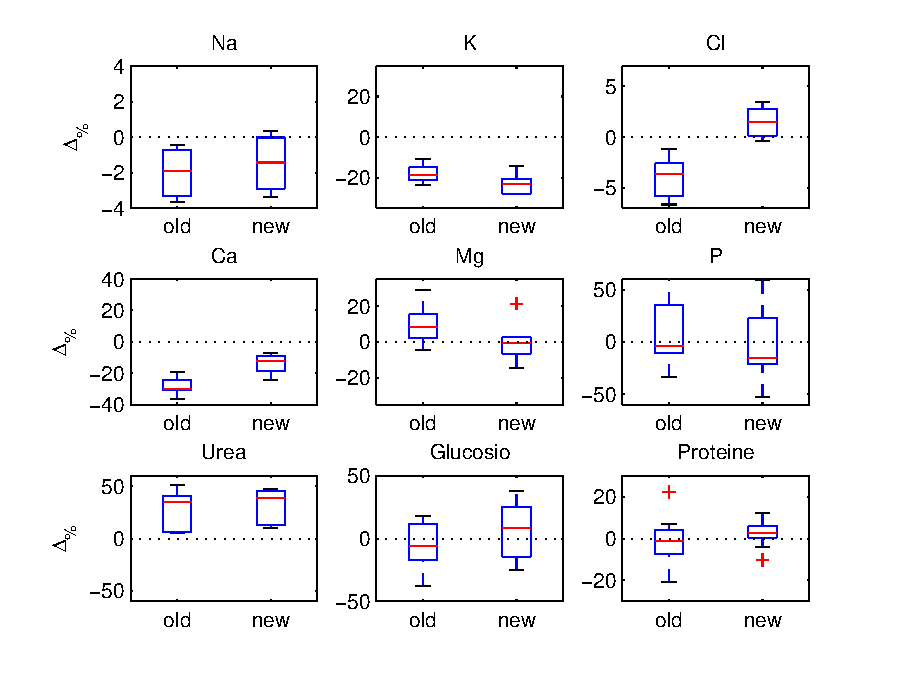
\includegraphics[width=\textwidth]{immagini/LUNIvsST.eps}
	\caption{Confronto fra modelli: variazione percentuale relativa ai dati di fine seduta. Boxplot calcolati coi dati di 10 sedute di pazienti diversi}
	\label{LUNIvsST}
\end{figure}
